\documentclass{standalone}
% \documentclass[12pt,a3paper]{article}
\usepackage{tikz}
\usetikzlibrary{math}

\begin{document}
\pagestyle{empty}

	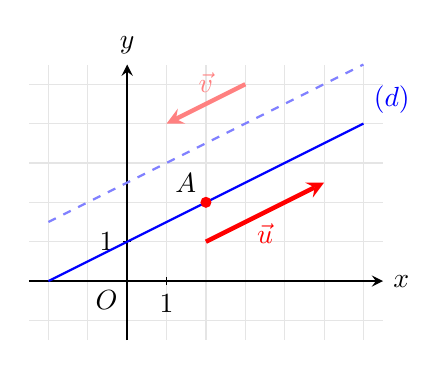
\begin{tikzpicture}[>=stealth, scale=0.5]
		% Grille pour la lisibilité
		\draw[thin, gray!20] (-2.5,-1.5) grid (6.5,5.5);

		% Axes gradués
		\draw[->, thick] (-2.5,0) -- (6.5,0) node[right] {$x$};
		\draw[->, thick] (0,-1.5) -- (0,5.5) node[above] {$y$};
		\draw (1,0.1) -- (1,-0.1) node[below] {$1$};
		\draw (0.1,1) -- (-0.1,1) node[left] {$1$};
		\node[below left] at (0,0) {$O$};

		% Dessin de la droite (équation y = 0.5x + 1)
		\draw[blue, thick] (-2,0) -- (6,4) node[above right] {$(d)$};
		\draw[blue!50!white, thick, dashed] (-2,1.5) -- (6,5.5);
		% \draw[lightgray, thick] (-2,4) -- (6,1);

		% Point A sur la droite
		\coordinate (A) at (2,2);
		\fill[red] (A) circle (4pt) node[above left, black] {$A$};

		% Vecteur directeur u (3 en x, 1.5 en y pour rester sur la droite)
		\coordinate (C) at (2,1);
		\coordinate (B) at (5,2.5);
		\draw[->, ultra thick, red] (C) -- (B) node[midway, below] {$\vec{u}$};
		\draw[->, ultra thick, red!50!white] (3,5) -- (1,4) node[midway, above] {$\vec{v}$};
	\end{tikzpicture}

\end{document}
